\begin{Example}[berkeley6]{Berkeley admissions}
The homogeneous association model $[AD] [GD] [AG]$, \eqref{eq:berk1}, may be fit as a generalized linear
model for log frequency with \PROC{GENMOD} as shown below, and produces the model fit
statistics shown in \outref{out:genberk2.1}.  The Deviance statistic is identical to
the \LR\ \GSQ\ shown in \outref{out:catberk5.1}.
The keywords \pname{type3 wald} give Type III Wald tests of individual terms,
similar to the maximum likelihood ANOVA table produced by \PROC{CATMOD}.
\begin{listing}
proc genmod data=berkeley;
   class dept gender admit;
   model freq = dept|gender|admit@2 / dist=poisson link=log type3 wald;
\end{listing}

\begin{Output}[htb]
\caption{Berkeley admissions data: Model [AD] [AG] [DG], fit with \PROC{GENMOD}}\label{out:genberk2.1}
\small
\verbatiminput{ch7/out/genberk2.1}
\end{Output}

We fit the model $[AD] [GD]$ as shown below.
This is the conditional independence model, $A \perp G \given D$.  Because this model does not
fit well, we obtain the residuals among the observation statistics
with the statement \pname{make 'obstats' out=obstats;}.
The factor variables \pname{dept gender admit} are merged with the \pname{obstats} \Dset,
translated to more meaningful labels, and
we request a mosaic display with the \macro{MOSAIC}.
\begin{listing}
proc genmod data=berkeley;
   class dept gender admit;
   model freq = admit|dept gender|dept / dist=poisson obstats residuals;
   make 'obstats' out=obstats;
data obstats;
   merge berkeley obstats;
   D = put(dept, dept.);
   if admit=1
      then A='Admitted';
      else A='Rejected';
   if gender='F'
      then G = 'Female';
      else G = 'Male';

%mosaic(data=obstats, var=A G D, vorder=A G D, count=freq,
   resid=streschi, cellfill=dev, split=H V,
   title=Model: [AdmitDept] [GenderDept]);
\end{listing}
The mosaic display, shown in \figref{fig:mosaic9a}, indicates that this model fits well
(residuals are small)
except in Department A.
%% one figure
\begin{figure}[htb]
  \centering
  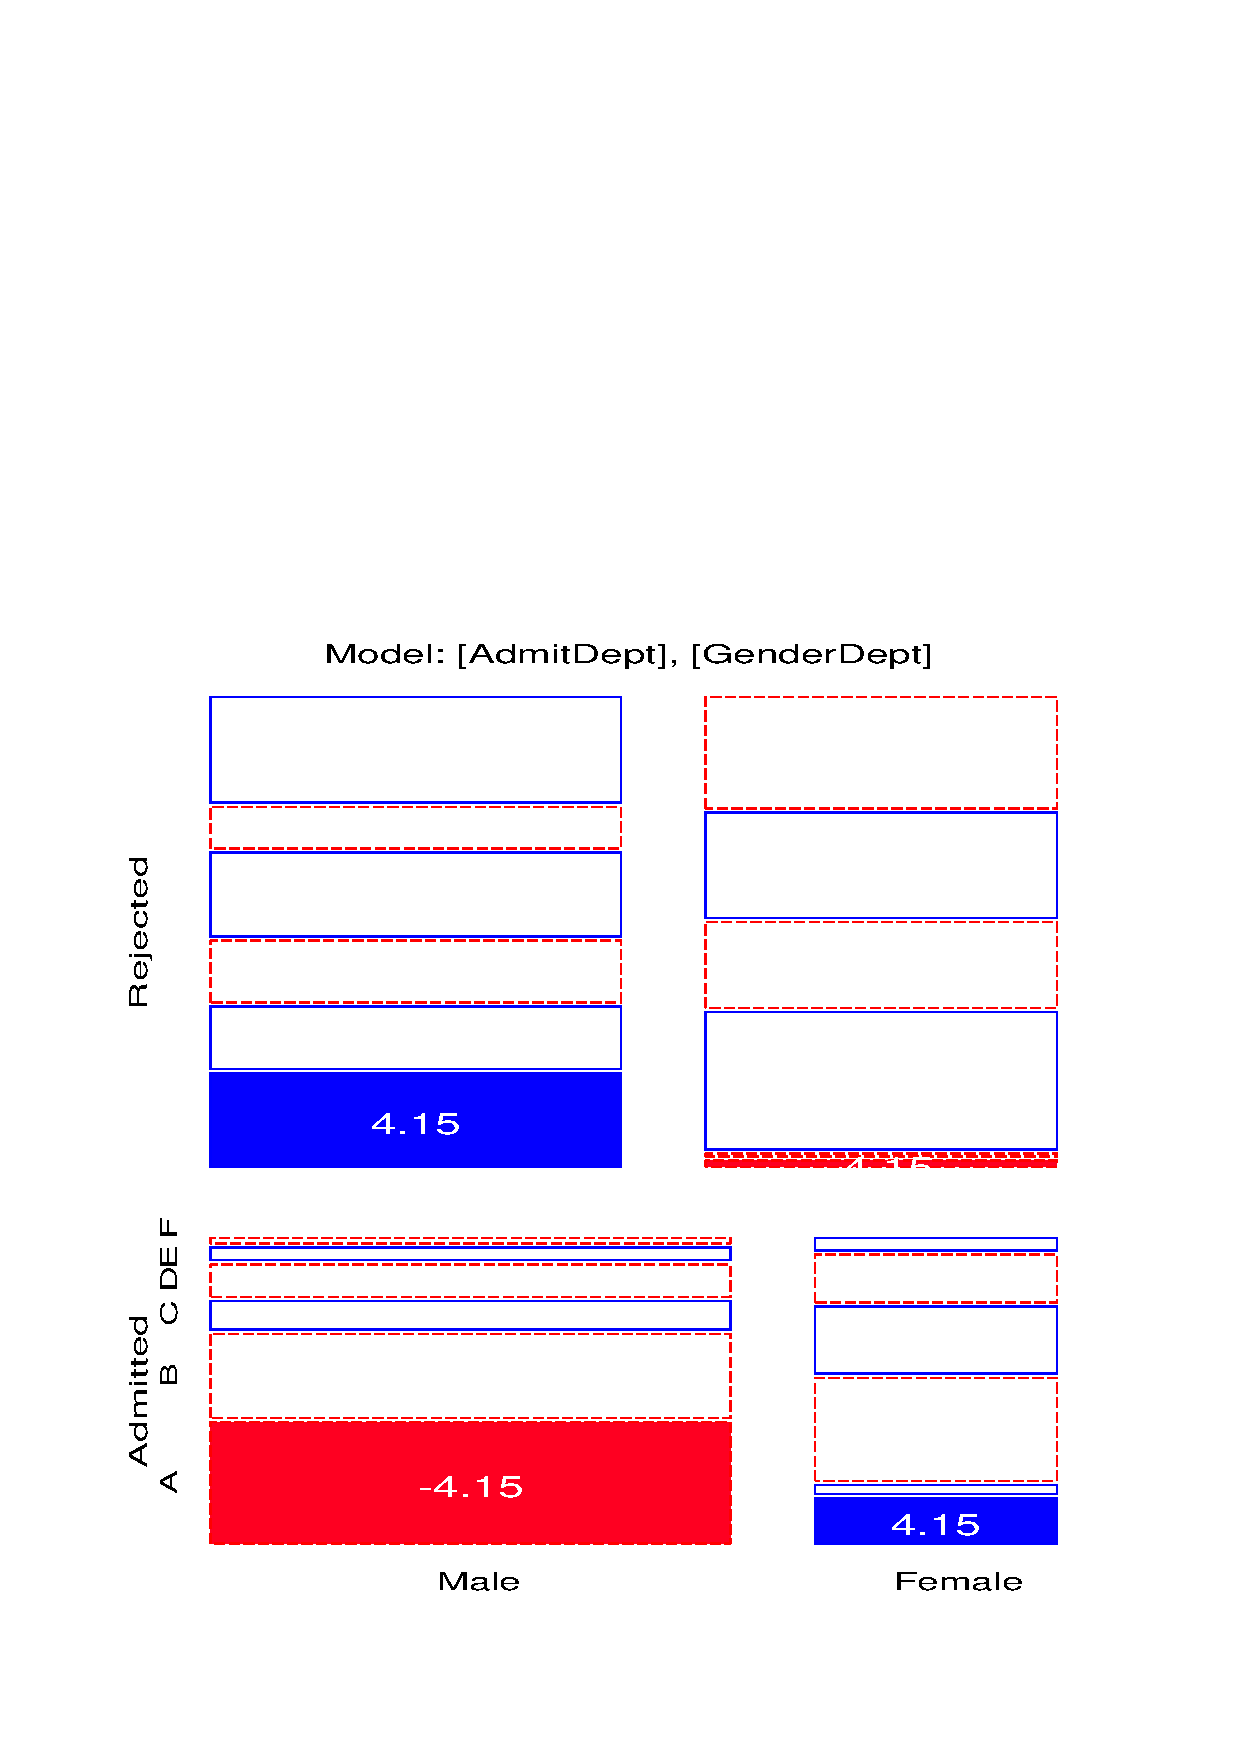
\includegraphics[scale=.6]{mosaic9a}
  \caption{Mosaic display for Berkeley admissions data}%
  \label{fig:mosaic9a}
\end{figure}
This suggests a model which allows an association between Admission and Gender in Department
A only,
\begin{equation}\label{eq:berk2}
  \log \,  m_{ijk}  =
  \mu
  +  \lambda_i^A
  +  \lambda_j^D
  +  \lambda_k^G
  +  \lambda_{ij}^{AD}
  +  \lambda_{jk}^{DG}
  +  \delta_{j=1} \lambda_{ik}^{AG} \comma
\end{equation}
where $\delta_{j=1}$ equals 1 for Department A ($j=1$) and is zero otherwise.
This model asserts that Admission and Gender are conditionally independent,
given Department, except in Department A.  It has one more parameter than
the conditional independence model, $[AD] [GD]$.
Model \eqref{eq:berk2} may be fit with \PROC{GENMOD} by constructing a variable
equal to the interaction of \pname{gender} and \pname{admit}
with a dummy variable having the value 1 for Department A and 0 for other departments.
\begin{listing}
data berkeley;
   set berkeley;
   dept1AG = (gender='F') * admit * (dept=1);

proc genmod data=berkeley;
   class dept gender admit;
   model freq = dept|gender dept|admit dept1AG / dist=poisson type3 wald;
\end{listing}
The model fit statistics and Type III tests for model \eqref{eq:berk2} are shown in
\outref{out:genberk2.2}.  This model fits very well indeed.
The parameter estimate, $\widehat{\lambda}_{ik}^{AG} = 1.052$ may be interpreted as
the log odds ratio of admission for females as compared to males in Dept. A.
The odds ratio is $\exp(1.052) = 2.86$, the same as the value calculated from the
raw data (see \secref{sec:twoway-fourstrat}).
\begin{Output}[htb]
\caption{Berkeley admissions data: Model \eqref{eq:berk2}, fit with \PROC{GENMOD}}\label{out:genberk2.2}
\small
\verbatiminput{ch7/out/genberk2.2}
\end{Output}
\end{Example}
